%% Generated by Sphinx.
\def\sphinxdocclass{report}
\documentclass[a4paper,10pt,english]{sphinxmanual}
\ifdefined\pdfpxdimen
   \let\sphinxpxdimen\pdfpxdimen\else\newdimen\sphinxpxdimen
\fi \sphinxpxdimen=.75bp\relax

\usepackage[utf8]{inputenc}
\ifdefined\DeclareUnicodeCharacter
 \ifdefined\DeclareUnicodeCharacterAsOptional
  \DeclareUnicodeCharacter{"00A0}{\nobreakspace}
  \DeclareUnicodeCharacter{"2500}{\sphinxunichar{2500}}
  \DeclareUnicodeCharacter{"2502}{\sphinxunichar{2502}}
  \DeclareUnicodeCharacter{"2514}{\sphinxunichar{2514}}
  \DeclareUnicodeCharacter{"251C}{\sphinxunichar{251C}}
  \DeclareUnicodeCharacter{"2572}{\textbackslash}
 \else
  \DeclareUnicodeCharacter{00A0}{\nobreakspace}
  \DeclareUnicodeCharacter{2500}{\sphinxunichar{2500}}
  \DeclareUnicodeCharacter{2502}{\sphinxunichar{2502}}
  \DeclareUnicodeCharacter{2514}{\sphinxunichar{2514}}
  \DeclareUnicodeCharacter{251C}{\sphinxunichar{251C}}
  \DeclareUnicodeCharacter{2572}{\textbackslash}
 \fi
\fi
\usepackage{cmap}
\usepackage[T1]{fontenc}
\usepackage{amsmath,amssymb,amstext}
\usepackage{babel}
\usepackage{times}
\usepackage[Bjarne]{fncychap}
\usepackage[dontkeepoldnames]{sphinx}

\usepackage{geometry}

% Include hyperref last.
\usepackage{hyperref}
% Fix anchor placement for figures with captions.
\usepackage{hypcap}% it must be loaded after hyperref.
% Set up styles of URL: it should be placed after hyperref.
\urlstyle{same}

\addto\captionsenglish{\renewcommand{\figurename}{Fig.}}
\addto\captionsenglish{\renewcommand{\tablename}{Table}}
\addto\captionsenglish{\renewcommand{\literalblockname}{Listing}}

\addto\captionsenglish{\renewcommand{\literalblockcontinuedname}{continued from previous page}}
\addto\captionsenglish{\renewcommand{\literalblockcontinuesname}{continues on next page}}

\addto\extrasenglish{\def\pageautorefname{page}}





\title{termtools Documentation}
\date{Feb 06, 2018}
\release{0.0.8}
\author{Yasser Mohammad}
\newcommand{\sphinxlogo}{\vbox{}}
\renewcommand{\releasename}{Release}
\makeindex

\begin{document}

\maketitle
\sphinxtableofcontents
\phantomsection\label{\detokenize{index::doc}}



\chapter{A set of terminal tools that helps building apps that look nice on the terminal}
\label{\detokenize{index:welcome-to-termtools-s-documentation}}\label{\detokenize{index:a-set-of-terminal-tools-that-helps-building-apps-that-look-nice-on-the-terminal}}
This is a simple library for controlling \sphinxstyleemphasis{text} appearance and placement
on terminals. It provides also an advanced progress bar library.

The main advantages of the progress bar library included here are the
following:
\begin{itemize}
\item {} 
Easily show multiple progress bars controlled independently

\item {} 
Control the placement of the bars anyplace on the screen

\item {} 
Control the appearance of the bars using a simple markup like
interface

\item {} 
When no information about the actual progress is available (which
happens alot in datascience applications), it is possible to just
indicate that the system is not stuck

\end{itemize}


\chapter{Table of Contents}
\label{\detokenize{index:table-of-contents}}

\section{Reference}
\label{\detokenize{references::doc}}\label{\detokenize{references:module-termtools.terminal}}\label{\detokenize{references:reference}}\index{termtools.terminal (module)}
This module exposes classes to control displaying text and progress bars at any place of the screen.

The two main classes are TerminalController and ProgressBarController


\subsection{Functions}
\label{\detokenize{references:functions}}

\begin{savenotes}\sphinxatlongtablestart\begin{longtable}{p{0.5\linewidth}p{0.5\linewidth}}
\hline

\endfirsthead

\multicolumn{2}{c}%
{\makebox[0pt]{\sphinxtablecontinued{\tablename\ \thetable{} -- continued from previous page}}}\\
\hline

\endhead

\hline
\multicolumn{2}{r}{\makebox[0pt][r]{\sphinxtablecontinued{Continued on next page}}}\\
\endfoot

\endlastfoot

\sphinxcode{humanize\_time}(secs{[}, align, …{]})
&
Prints time that is given as seconds in human readable form.
\\
\hline
\sphinxcode{print\_progress}(iteration, total{[}, prefix, …{]})
&
Call in a loop to create terminal progress bar
\\
\hline
\end{longtable}\sphinxatlongtableend\end{savenotes}


\subsubsection{humanize\_time}
\label{\detokenize{api/termtools.terminal.humanize_time::doc}}\label{\detokenize{api/termtools.terminal.humanize_time:humanize-time}}\index{humanize\_time() (in module termtools.terminal)}

\begin{fulllineitems}
\phantomsection\label{\detokenize{api/termtools.terminal.humanize_time:termtools.terminal.humanize_time}}\pysiglinewithargsret{\sphinxcode{termtools.terminal.}\sphinxbfcode{humanize\_time}}{\emph{secs}, \emph{align=False}, \emph{always\_show\_all\_units=False}}{}
Prints time that is given as seconds in human readable form. Useful only for times \textgreater{}=1sec.
\begin{quote}\begin{description}
\item[{Parameters}] \leavevmode\begin{itemize}
\item {} 
\sphinxstyleliteralstrong{float} (\sphinxstyleliteralemphasis{secs}) \textendash{} number of seconds

\item {} 
\sphinxstyleliteralstrong{bool}\sphinxstyleliteralstrong{, }\sphinxstyleliteralstrong{optional} (\sphinxstyleliteralemphasis{always\_show\_all\_units}) \textendash{} whether to align outputs so that they all take the same size (not implemented)

\item {} 
\sphinxstyleliteralstrong{bool}\sphinxstyleliteralstrong{, }\sphinxstyleliteralstrong{optional} \textendash{} Whether to always show days, hours, and minutes even when they
are zeros. default False

\end{itemize}

\item[{Returns}] \leavevmode
str formated string with the humanized form

\end{description}\end{quote}

\end{fulllineitems}



\subsubsection{print\_progress}
\label{\detokenize{api/termtools.terminal.print_progress::doc}}\label{\detokenize{api/termtools.terminal.print_progress:print-progress}}\index{print\_progress() (in module termtools.terminal)}

\begin{fulllineitems}
\phantomsection\label{\detokenize{api/termtools.terminal.print_progress:termtools.terminal.print_progress}}\pysiglinewithargsret{\sphinxcode{termtools.terminal.}\sphinxbfcode{print\_progress}}{\emph{iteration}, \emph{total}, \emph{prefix=''}, \emph{suffix=''}, \emph{decimals=2}, \emph{barLength=50}, \emph{limit\_range=True}}{}
Call in a loop to create terminal progress bar
\begin{quote}\begin{description}
\item[{Parameters}] \leavevmode\begin{itemize}
\item {} 
\sphinxstyleliteralstrong{int} (\sphinxstyleliteralemphasis{barLength}) \textendash{} current iteration

\item {} 
\sphinxstyleliteralstrong{int} \textendash{} total iterations

\item {} 
\sphinxstyleliteralstrong{str} (\sphinxstyleliteralemphasis{suffix}) \textendash{} prefix string

\item {} 
\sphinxstyleliteralstrong{str} \textendash{} suffix string

\item {} 
\sphinxstyleliteralstrong{int} \textendash{} positive number of decimals in percent complete

\item {} 
\sphinxstyleliteralstrong{int} \textendash{} character length of bar

\end{itemize}

\end{description}\end{quote}

\end{fulllineitems}



\subsection{Classes}
\label{\detokenize{references:classes}}

\begin{savenotes}\sphinxatlongtablestart\begin{longtable}{p{0.5\linewidth}p{0.5\linewidth}}
\hline

\endfirsthead

\multicolumn{2}{c}%
{\makebox[0pt]{\sphinxtablecontinued{\tablename\ \thetable{} -- continued from previous page}}}\\
\hline

\endhead

\hline
\multicolumn{2}{r}{\makebox[0pt][r]{\sphinxtablecontinued{Continued on next page}}}\\
\endfoot

\endlastfoot

\sphinxcode{ProgressBarController}({[}barNames, barLength, …{]})
&
A set of progress bars.
\\
\hline
\sphinxcode{TerminalController}()
&
A class for controlling where to print on a screen and the attributes of text to be printed.
\\
\hline
\end{longtable}\sphinxatlongtableend\end{savenotes}


\subsubsection{ProgressBarController}
\label{\detokenize{api/termtools.terminal.ProgressBarController::doc}}\label{\detokenize{api/termtools.terminal.ProgressBarController:progressbarcontroller}}\index{ProgressBarController (class in termtools.terminal)}

\begin{fulllineitems}
\phantomsection\label{\detokenize{api/termtools.terminal.ProgressBarController:termtools.terminal.ProgressBarController}}\pysiglinewithargsret{\sphinxbfcode{class }\sphinxcode{termtools.terminal.}\sphinxbfcode{ProgressBarController}}{\emph{barNames=None}, \emph{barLength=50}, \emph{align\_bars=True}}{}
Bases: \sphinxcode{object}

A set of progress bars.

A set of progress bars with custom pre and post text. It is mostly useful when you have several running threads or
suprocesses and each needs its own bar. It allows prefixes and postfixes that can be changed using the following tags:
\textless{}name\textgreater{} bar name
\textless{}remaining\textgreater{} remaining time to completion estimate
\textless{}activity\textgreater{} An indicator that the process represented by the bar is active
\paragraph{Attributes Summary}


\begin{savenotes}\sphinxatlongtablestart\begin{longtable}{p{0.5\linewidth}p{0.5\linewidth}}
\hline

\endfirsthead

\multicolumn{2}{c}%
{\makebox[0pt]{\sphinxtablecontinued{\tablename\ \thetable{} -- continued from previous page}}}\\
\hline

\endhead

\hline
\multicolumn{2}{r}{\makebox[0pt][r]{\sphinxtablecontinued{Continued on next page}}}\\
\endfoot

\endlastfoot

\sphinxcode{activityChars}
&

\\
\hline
\sphinxcode{barNames}
&

\\
\hline
\sphinxcode{begTime}
&

\\
\hline
\sphinxcode{completed\_background}
&

\\
\hline
\sphinxcode{completed\_color}
&

\\
\hline
\sphinxcode{current}
&

\\
\hline
\sphinxcode{last\_i}
&

\\
\hline
\sphinxcode{last\_n}
&

\\
\hline
\sphinxcode{last\_name\_updated}
&

\\
\hline
\sphinxcode{over\_complete\_background}
&

\\
\hline
\sphinxcode{over\_complete\_color}
&

\\
\hline
\sphinxcode{running\_background}
&

\\
\hline
\sphinxcode{running\_color}
&

\\
\hline
\sphinxcode{under\_complete\_background}
&

\\
\hline
\sphinxcode{under\_complete\_color}
&

\\
\hline
\end{longtable}\sphinxatlongtableend\end{savenotes}
\paragraph{Methods Summary}


\begin{savenotes}\sphinxatlongtablestart\begin{longtable}{p{0.5\linewidth}p{0.5\linewidth}}
\hline

\endfirsthead

\multicolumn{2}{c}%
{\makebox[0pt]{\sphinxtablecontinued{\tablename\ \thetable{} -- continued from previous page}}}\\
\hline

\endhead

\hline
\multicolumn{2}{r}{\makebox[0pt][r]{\sphinxtablecontinued{Continued on next page}}}\\
\endfoot

\endlastfoot

\sphinxcode{activate}({[}name{]})
&
Indicate that the given bar is active.
\\
\hline
\sphinxcode{add\_bar}(name, *{[}, i, n, start\_timing{]})
&
Adds a bar
\\
\hline
\sphinxcode{get\_remaining\_time}(name)
&
Gets the time remaining till the end of execution (only an estimate)
\\
\hline
\sphinxcode{remove\_bar}(name)
&
Removes a bar given its name
\\
\hline
\sphinxcode{set\_progress}(name, i{[}, n{]})
&
Sets progress for a specific bar, optionally setting its limit as well
\\
\hline
\sphinxcode{show}({[}name, prefix, suffix, bar\_length, …{]})
&
Shows a specific bar just in the current place on the screen.
\\
\hline
\sphinxcode{show\_all}({[}barname, i, n, clean\_screen, …{]})
&
Shows a specific bar or all bars, possibly cleaning the screen
\\
\hline
\sphinxcode{show\_in\_position}({[}name, prefix, suffix, …{]})
&
Shows the named bar in its appropriate position without touching anything else in the screen
\\
\hline
\sphinxcode{start\_timing}({[}forNames{]})
&
Starts timing for ETA calculation for the given bar names
\\
\hline
\sphinxcode{terminal}()
&
Gets the built-in \sphinxtitleref{TerminalController} object
\\
\hline
\sphinxcode{update}({[}name, i, n, prefix, suffix, bar\_length{]})
&
Updates the progress value of a given bar and shows all the bars in their relative positions
\\
\hline
\end{longtable}\sphinxatlongtableend\end{savenotes}
\paragraph{Attributes Documentation}
\index{activityChars (termtools.terminal.ProgressBarController attribute)}

\begin{fulllineitems}
\phantomsection\label{\detokenize{api/termtools.terminal.ProgressBarController:termtools.terminal.ProgressBarController.activityChars}}\pysigline{\sphinxbfcode{activityChars}\sphinxbfcode{ = {[}'.   ', ' .  ', '  . ', '   .', '  . ', ' .  ', '.   '{]}}}
\end{fulllineitems}

\index{barNames (termtools.terminal.ProgressBarController attribute)}

\begin{fulllineitems}
\phantomsection\label{\detokenize{api/termtools.terminal.ProgressBarController:termtools.terminal.ProgressBarController.barNames}}\pysigline{\sphinxbfcode{barNames}\sphinxbfcode{ = None}}
\end{fulllineitems}

\index{begTime (termtools.terminal.ProgressBarController attribute)}

\begin{fulllineitems}
\phantomsection\label{\detokenize{api/termtools.terminal.ProgressBarController:termtools.terminal.ProgressBarController.begTime}}\pysigline{\sphinxbfcode{begTime}\sphinxbfcode{ = None}}
\end{fulllineitems}

\index{completed\_background (termtools.terminal.ProgressBarController attribute)}

\begin{fulllineitems}
\phantomsection\label{\detokenize{api/termtools.terminal.ProgressBarController:termtools.terminal.ProgressBarController.completed_background}}\pysigline{\sphinxbfcode{completed\_background}\sphinxbfcode{ = 'black'}}
\end{fulllineitems}

\index{completed\_color (termtools.terminal.ProgressBarController attribute)}

\begin{fulllineitems}
\phantomsection\label{\detokenize{api/termtools.terminal.ProgressBarController:termtools.terminal.ProgressBarController.completed_color}}\pysigline{\sphinxbfcode{completed\_color}\sphinxbfcode{ = 'green'}}
\end{fulllineitems}

\index{current (termtools.terminal.ProgressBarController attribute)}

\begin{fulllineitems}
\phantomsection\label{\detokenize{api/termtools.terminal.ProgressBarController:termtools.terminal.ProgressBarController.current}}\pysigline{\sphinxbfcode{current}\sphinxbfcode{ = None}}
\end{fulllineitems}

\index{last\_i (termtools.terminal.ProgressBarController attribute)}

\begin{fulllineitems}
\phantomsection\label{\detokenize{api/termtools.terminal.ProgressBarController:termtools.terminal.ProgressBarController.last_i}}\pysigline{\sphinxbfcode{last\_i}\sphinxbfcode{ = None}}
\end{fulllineitems}

\index{last\_n (termtools.terminal.ProgressBarController attribute)}

\begin{fulllineitems}
\phantomsection\label{\detokenize{api/termtools.terminal.ProgressBarController:termtools.terminal.ProgressBarController.last_n}}\pysigline{\sphinxbfcode{last\_n}\sphinxbfcode{ = None}}
\end{fulllineitems}

\index{last\_name\_updated (termtools.terminal.ProgressBarController attribute)}

\begin{fulllineitems}
\phantomsection\label{\detokenize{api/termtools.terminal.ProgressBarController:termtools.terminal.ProgressBarController.last_name_updated}}\pysigline{\sphinxbfcode{last\_name\_updated}\sphinxbfcode{ = None}}
\end{fulllineitems}

\index{over\_complete\_background (termtools.terminal.ProgressBarController attribute)}

\begin{fulllineitems}
\phantomsection\label{\detokenize{api/termtools.terminal.ProgressBarController:termtools.terminal.ProgressBarController.over_complete_background}}\pysigline{\sphinxbfcode{over\_complete\_background}\sphinxbfcode{ = 'black'}}
\end{fulllineitems}

\index{over\_complete\_color (termtools.terminal.ProgressBarController attribute)}

\begin{fulllineitems}
\phantomsection\label{\detokenize{api/termtools.terminal.ProgressBarController:termtools.terminal.ProgressBarController.over_complete_color}}\pysigline{\sphinxbfcode{over\_complete\_color}\sphinxbfcode{ = 'red'}}
\end{fulllineitems}

\index{running\_background (termtools.terminal.ProgressBarController attribute)}

\begin{fulllineitems}
\phantomsection\label{\detokenize{api/termtools.terminal.ProgressBarController:termtools.terminal.ProgressBarController.running_background}}\pysigline{\sphinxbfcode{running\_background}\sphinxbfcode{ = 'black'}}
\end{fulllineitems}

\index{running\_color (termtools.terminal.ProgressBarController attribute)}

\begin{fulllineitems}
\phantomsection\label{\detokenize{api/termtools.terminal.ProgressBarController:termtools.terminal.ProgressBarController.running_color}}\pysigline{\sphinxbfcode{running\_color}\sphinxbfcode{ = 'yellow'}}
\end{fulllineitems}

\index{under\_complete\_background (termtools.terminal.ProgressBarController attribute)}

\begin{fulllineitems}
\phantomsection\label{\detokenize{api/termtools.terminal.ProgressBarController:termtools.terminal.ProgressBarController.under_complete_background}}\pysigline{\sphinxbfcode{under\_complete\_background}\sphinxbfcode{ = 'black'}}
\end{fulllineitems}

\index{under\_complete\_color (termtools.terminal.ProgressBarController attribute)}

\begin{fulllineitems}
\phantomsection\label{\detokenize{api/termtools.terminal.ProgressBarController:termtools.terminal.ProgressBarController.under_complete_color}}\pysigline{\sphinxbfcode{under\_complete\_color}\sphinxbfcode{ = 'red'}}
\end{fulllineitems}

\paragraph{Methods Documentation}
\index{activate() (termtools.terminal.ProgressBarController method)}

\begin{fulllineitems}
\phantomsection\label{\detokenize{api/termtools.terminal.ProgressBarController:termtools.terminal.ProgressBarController.activate}}\pysiglinewithargsret{\sphinxbfcode{activate}}{\emph{name=None}}{}
Indicate that the given bar is active. If name is None, all bars are indicated to be active by progressing
\begin{quote}\begin{description}
\item[{Parameters}] \leavevmode
\sphinxstyleliteralstrong{name} (\sphinxstyleliteralemphasis{str}) \textendash{} bar name. If None is given then all bars are set to be active

\item[{Returns}] \leavevmode
self

\end{description}\end{quote}

\end{fulllineitems}

\index{add\_bar() (termtools.terminal.ProgressBarController method)}

\begin{fulllineitems}
\phantomsection\label{\detokenize{api/termtools.terminal.ProgressBarController:termtools.terminal.ProgressBarController.add_bar}}\pysiglinewithargsret{\sphinxbfcode{add\_bar}}{\emph{name}, \emph{*}, \emph{i=0}, \emph{n=0}, \emph{start\_timing=True}}{}
Adds a bar

Can control the name, starting progress (i) and total progress
\begin{quote}\begin{description}
\item[{Parameters}] \leavevmode
\sphinxstyleliteralstrong{name} (\sphinxstyleliteralemphasis{str}) \textendash{} name of bar

\end{description}\end{quote}
\begin{description}
\item[{Kwargs:}] \leavevmode
i (int): current progress
n (int): total progress
start\_timing (bool or None): Starts a timer for this bar, otherwise it uses the begTime member which
\begin{quote}

is common to all bars
\end{quote}

\end{description}
\begin{quote}\begin{description}
\item[{Returns}] \leavevmode
self

\end{description}\end{quote}

Remarks:

\end{fulllineitems}

\index{get\_remaining\_time() (termtools.terminal.ProgressBarController method)}

\begin{fulllineitems}
\phantomsection\label{\detokenize{api/termtools.terminal.ProgressBarController:termtools.terminal.ProgressBarController.get_remaining_time}}\pysiglinewithargsret{\sphinxbfcode{get\_remaining\_time}}{\emph{name}}{}
Gets the time remaining till the end of execution (only an estimate)
\begin{quote}\begin{description}
\item[{Parameters}] \leavevmode
\sphinxstyleliteralstrong{name} \textendash{} bar name

\item[{Returns}] \leavevmode
remaining time (ETA)

\item[{Return type}] \leavevmode
int

\end{description}\end{quote}

\end{fulllineitems}

\index{remove\_bar() (termtools.terminal.ProgressBarController method)}

\begin{fulllineitems}
\phantomsection\label{\detokenize{api/termtools.terminal.ProgressBarController:termtools.terminal.ProgressBarController.remove_bar}}\pysiglinewithargsret{\sphinxbfcode{remove\_bar}}{\emph{name}}{}
Removes a bar given its name
\begin{quote}\begin{description}
\item[{Parameters}] \leavevmode
\sphinxstyleliteralstrong{name} (\sphinxstyleliteralemphasis{str}) \textendash{} bar name

\item[{Returns}] \leavevmode
self

\end{description}\end{quote}

\end{fulllineitems}

\index{set\_progress() (termtools.terminal.ProgressBarController method)}

\begin{fulllineitems}
\phantomsection\label{\detokenize{api/termtools.terminal.ProgressBarController:termtools.terminal.ProgressBarController.set_progress}}\pysiglinewithargsret{\sphinxbfcode{set\_progress}}{\emph{name}, \emph{i}, \emph{n=None}}{}
Sets progress for a specific bar, optionally setting its limit as well
\begin{quote}\begin{description}
\item[{Parameters}] \leavevmode\begin{itemize}
\item {} 
\sphinxstyleliteralstrong{name} (\sphinxstyleliteralemphasis{str}) \textendash{} bar name

\item {} 
\sphinxstyleliteralstrong{i} (\sphinxstyleliteralemphasis{int}) \textendash{} current progress

\item {} 
\sphinxstyleliteralstrong{n} (\sphinxstyleliteralemphasis{int}\sphinxstyleliteralemphasis{ or }\sphinxstyleliteralemphasis{None}) \textendash{} Limit (optional)

\end{itemize}

\item[{Returns}] \leavevmode
self

\end{description}\end{quote}

\end{fulllineitems}

\index{show() (termtools.terminal.ProgressBarController method)}

\begin{fulllineitems}
\phantomsection\label{\detokenize{api/termtools.terminal.ProgressBarController:termtools.terminal.ProgressBarController.show}}\pysiglinewithargsret{\sphinxbfcode{show}}{\emph{name=None}, \emph{prefix='\textless{}name\textgreater{}'}, \emph{suffix='\textless{}remaining\textgreater{}'}, \emph{bar\_length=-1}, \emph{from\_line\_beginning=True}}{}
Shows a specific bar just in the current place on the screen. We should have a new line before it
\begin{quote}
\begin{description}
\item[{Args:}] \leavevmode
name (str or None): name of the bar
prefix (str): prefix to write before the bar (see the class doc string for possible tag values)
suffix (str): postfix (see prefix)
bar\_length (int): Bar length, if less than zero then the current length set during creation of the bar or
\begin{quote}

latest setting of its progess will be used.
\end{quote}

from\_line\_beginning (bool): If true, a ‘

\end{description}
\end{quote}
\begin{description}
\item[{‘ and flushing will be outputed to set the bar to the beginning}] \leavevmode\begin{quote}

of the line
\end{quote}
\begin{description}
\item[{Returns:}] \leavevmode
self

\end{description}

\end{description}

\end{fulllineitems}

\index{show\_all() (termtools.terminal.ProgressBarController method)}

\begin{fulllineitems}
\phantomsection\label{\detokenize{api/termtools.terminal.ProgressBarController:termtools.terminal.ProgressBarController.show_all}}\pysiglinewithargsret{\sphinxbfcode{show\_all}}{\emph{barname=None}, \emph{i=None}, \emph{n=None}, \emph{clean\_screen=True}, \emph{prefix='\textless{}name\textgreater{}\textless{}activity\textgreater{}'}, \emph{suffix='\textless{}remaining\textgreater{}'}, \emph{bar\_length=-1}, \emph{skip\_rows=0}}{}
Shows a specific bar or all bars, possibly cleaning the screen
\begin{quote}\begin{description}
\item[{Parameters}] \leavevmode\begin{itemize}
\item {} 
\sphinxstyleliteralstrong{barname} (\sphinxstyleliteralemphasis{str}\sphinxstyleliteralemphasis{ or }\sphinxstyleliteralemphasis{None}) \textendash{} name of the bar

\item {} 
\sphinxstyleliteralstrong{i} (\sphinxstyleliteralemphasis{int}\sphinxstyleliteralemphasis{ or }\sphinxstyleliteralemphasis{None}) \textendash{} optional progress value

\item {} 
\sphinxstyleliteralstrong{n} (\sphinxstyleliteralemphasis{int}\sphinxstyleliteralemphasis{ or }\sphinxstyleliteralemphasis{None}) \textendash{} optional maximum value for the bar

\item {} 
\sphinxstyleliteralstrong{clean\_screen} (\sphinxstyleliteralemphasis{bool}) \textendash{} Whether or not to clean the screen before drawing. Default is true

\item {} 
\sphinxstyleliteralstrong{prefix} (\sphinxstyleliteralemphasis{str}) \textendash{} prefix to write before the bar (see the class doc string for possible tag values)

\item {} 
\sphinxstyleliteralstrong{suffix} (\sphinxstyleliteralemphasis{str}) \textendash{} postfix (see prefix)

\item {} 
\sphinxstyleliteralstrong{bar\_length} (\sphinxstyleliteralemphasis{int}) \textendash{} Bar length, if less than zero then the current length set during creation of the bar or latest setting of its progess will be used.

\item {} 
\sphinxstyleliteralstrong{skip\_rows} (\sphinxstyleliteralemphasis{int}) \textendash{} the number of lines to skip between bars

\item {} 
\sphinxstyleliteralstrong{from\_line\_beginning} (\sphinxstyleliteralemphasis{bool}) \textendash{} If true, a r and flushing will be outputed to set the bar to the beginning of the line

\end{itemize}

\item[{Returns}] \leavevmode
self

\end{description}\end{quote}

Remarks:

\end{fulllineitems}

\index{show\_in\_position() (termtools.terminal.ProgressBarController method)}

\begin{fulllineitems}
\phantomsection\label{\detokenize{api/termtools.terminal.ProgressBarController:termtools.terminal.ProgressBarController.show_in_position}}\pysiglinewithargsret{\sphinxbfcode{show\_in\_position}}{\emph{name=None}, \emph{prefix='\textless{}name\textgreater{}\textless{}activity\textgreater{}'}, \emph{suffix='\textless{}remaining\textgreater{}'}, \emph{bar\_length=-1}}{}
Shows the named bar in its appropriate position without touching anything else in the screen
\begin{quote}\begin{description}
\item[{Parameters}] \leavevmode\begin{itemize}
\item {} 
\sphinxstyleliteralstrong{name} (\sphinxstyleliteralemphasis{str}) \textendash{} bar name

\item {} 
\sphinxstyleliteralstrong{clean\_screen} (\sphinxstyleliteralemphasis{bool}) \textendash{} Whether or not to clean the screen before drawing. Default is true

\item {} 
\sphinxstyleliteralstrong{prefix} (\sphinxstyleliteralemphasis{str}) \textendash{} prefix to write before the bar (see the class doc string for possible tag values)

\item {} 
\sphinxstyleliteralstrong{suffix} (\sphinxstyleliteralemphasis{str}) \textendash{} postfix (see prefix)

\item {} 
\sphinxstyleliteralstrong{bar\_length} (\sphinxstyleliteralemphasis{int}) \textendash{} Bar length, if less than zero then the current length set during creation of the bar or
latest setting of its progress will be used.

\end{itemize}

\item[{Returns}] \leavevmode
self

\end{description}\end{quote}

\end{fulllineitems}

\index{start\_timing() (termtools.terminal.ProgressBarController method)}

\begin{fulllineitems}
\phantomsection\label{\detokenize{api/termtools.terminal.ProgressBarController:termtools.terminal.ProgressBarController.start_timing}}\pysiglinewithargsret{\sphinxbfcode{start\_timing}}{\emph{forNames=None}}{}
Starts timing for ETA calculation for the given bar names
\begin{quote}\begin{description}
\item[{Parameters}] \leavevmode
\sphinxstyleliteralstrong{forNames} (\sphinxstyleliteralemphasis{str}\sphinxstyleliteralemphasis{ or }\sphinxstyleliteralemphasis{None}) \textendash{} The list of bar names. If None (Default), the beginning time of all bars is set to
now

\item[{Returns}] \leavevmode
self

\end{description}\end{quote}

\end{fulllineitems}

\index{terminal() (termtools.terminal.ProgressBarController method)}

\begin{fulllineitems}
\phantomsection\label{\detokenize{api/termtools.terminal.ProgressBarController:termtools.terminal.ProgressBarController.terminal}}\pysiglinewithargsret{\sphinxbfcode{terminal}}{}{}
Gets the built-in \sphinxtitleref{TerminalController} object
\begin{quote}\begin{description}
\item[{Return type}] \leavevmode
\sphinxcode{TerminalController}

\item[{Returns}] \leavevmode
TerminalController

\end{description}\end{quote}

\end{fulllineitems}

\index{update() (termtools.terminal.ProgressBarController method)}

\begin{fulllineitems}
\phantomsection\label{\detokenize{api/termtools.terminal.ProgressBarController:termtools.terminal.ProgressBarController.update}}\pysiglinewithargsret{\sphinxbfcode{update}}{\emph{name=None}, \emph{i=None}, \emph{n=None}, \emph{prefix='\textless{}name\textgreater{}\textless{}activity\textgreater{}'}, \emph{suffix='\textless{}remaining\textgreater{}'}, \emph{bar\_length=-1}}{}
Updates the progress value of a given bar and shows all the bars in their relative positions
\begin{quote}\begin{description}
\item[{Parameters}] \leavevmode\begin{itemize}
\item {} 
\sphinxstyleliteralstrong{name} (\sphinxstyleliteralemphasis{str}) \textendash{} bar name

\item {} 
\sphinxstyleliteralstrong{i} (\sphinxstyleliteralemphasis{int}\sphinxstyleliteralemphasis{ or }\sphinxstyleliteralemphasis{None}) \textendash{} optional progress value

\item {} 
\sphinxstyleliteralstrong{n} (\sphinxstyleliteralemphasis{int}\sphinxstyleliteralemphasis{ or }\sphinxstyleliteralemphasis{None}) \textendash{} optional maximum value for the bar

\item {} 
\sphinxstyleliteralstrong{clean\_screen} (\sphinxstyleliteralemphasis{bool}) \textendash{} Whether or not to clean the screen before drawing. Default is true

\item {} 
\sphinxstyleliteralstrong{prefix} (\sphinxstyleliteralemphasis{str}) \textendash{} prefix to write before the bar (see the class doc string for possible tag values)

\item {} 
\sphinxstyleliteralstrong{suffix} (\sphinxstyleliteralemphasis{str}) \textendash{} postfix (see prefix)

\item {} 
\sphinxstyleliteralstrong{bar\_length} (\sphinxstyleliteralemphasis{int}) \textendash{} Bar length, if less than zero then the current length set during creation of the bar or
latest setting of its progess will be used.

\end{itemize}

\item[{Returns}] \leavevmode
self

\end{description}\end{quote}

\end{fulllineitems}


\end{fulllineitems}



\subsubsection{TerminalController}
\label{\detokenize{api/termtools.terminal.TerminalController::doc}}\label{\detokenize{api/termtools.terminal.TerminalController:terminalcontroller}}\index{TerminalController (class in termtools.terminal)}

\begin{fulllineitems}
\phantomsection\label{\detokenize{api/termtools.terminal.TerminalController:termtools.terminal.TerminalController}}\pysigline{\sphinxbfcode{class }\sphinxcode{termtools.terminal.}\sphinxbfcode{TerminalController}}
Bases: \sphinxcode{object}

A class for controlling where to print on a screen and the attributes of text to be printed.
\paragraph{Methods Summary}


\begin{savenotes}\sphinxatlongtablestart\begin{longtable}{p{0.5\linewidth}p{0.5\linewidth}}
\hline

\endfirsthead

\multicolumn{2}{c}%
{\makebox[0pt]{\sphinxtablecontinued{\tablename\ \thetable{} -- continued from previous page}}}\\
\hline

\endhead

\hline
\multicolumn{2}{r}{\makebox[0pt][r]{\sphinxtablecontinued{Continued on next page}}}\\
\endfoot

\endlastfoot

\sphinxcode{attrib}({[}attrib{]})
&
sets the text attributes
\\
\hline
\sphinxcode{background}({[}background{]})
&
sets the text background color
\\
\hline
\sphinxcode{bookmark}()
&
saves current cursor position
\\
\hline
\sphinxcode{clear}()
&
clears the screen
\\
\hline
\sphinxcode{color}({[}color{]})
&
sets the text foreground color
\\
\hline
\sphinxcode{down}({[}n{]})
&
goes down the specified number of rows
\\
\hline
\sphinxcode{eraseDown}()
&
erases all text from currnt line to the end of the screen
\\
\hline
\sphinxcode{eraseLine}()
&
erases all text from currnt line
\\
\hline
\sphinxcode{eraseToBOL}()
&
erases all text from currnt location to the beginning of the line
\\
\hline
\sphinxcode{eraseToEOL}()
&
erases all text from currnt location to the end of the line
\\
\hline
\sphinxcode{eraseUp}()
&
erases all text from currnt line to the beginning of the screen
\\
\hline
\sphinxcode{goto}({[}x, y{]})
&
goes to the specified x-y coordingates on the screen
\\
\hline
\sphinxcode{goto\_bookmark}()
&
goes to current bookmarked position (must use bookmark() before it)
\\
\hline
\sphinxcode{home}({[}erase\_screen{]})
&
gets the cursor to the top of the screen
\\
\hline
\sphinxcode{left}({[}n{]})
&
goes left the specified number of rows
\\
\hline
\sphinxcode{print}(*args, **kwargs)
&

\\
\hline
\sphinxcode{printat}(txt{[}, x, y{]})
&
goes to the specified x-y coordingates on the screen and prints the text.
\\
\hline
\sphinxcode{reset\_attributes}()
&
resets all text attributes to their defaults
\\
\hline
\sphinxcode{right}({[}n{]})
&
goes right the specified number of rows
\\
\hline
\sphinxcode{set\_attribute}({[}attrib{]})
&
sets the text attributes
\\
\hline
\sphinxcode{set\_attributes}({[}color, background, attrib{]})
&
sets the text attributes to be used by new prints. a value of “keep” keeps the current set
\\
\hline
\sphinxcode{set\_background}({[}background{]})
&
sets the text background color
\\
\hline
\sphinxcode{set\_foreground}({[}color{]})
&
sets the text foreground color
\\
\hline
\sphinxcode{up}({[}n{]})
&
goes up the specified number of rows
\\
\hline
\end{longtable}\sphinxatlongtableend\end{savenotes}
\paragraph{Methods Documentation}
\index{attrib() (termtools.terminal.TerminalController method)}

\begin{fulllineitems}
\phantomsection\label{\detokenize{api/termtools.terminal.TerminalController:termtools.terminal.TerminalController.attrib}}\pysiglinewithargsret{\sphinxbfcode{attrib}}{\emph{attrib='keep'}}{}~\begin{quote}

sets the text attributes
\end{quote}
\begin{quote}\begin{description}
\item[{Parameters}] \leavevmode
\sphinxstyleliteralstrong{attrib} \textendash{} one of {[}‘bright’,’dim’,’underscore’,’blink’,’reverse’,’hidden’{]}

\item[{Return type}] \leavevmode
TerminalController

\end{description}\end{quote}

\end{fulllineitems}

\index{background() (termtools.terminal.TerminalController method)}

\begin{fulllineitems}
\phantomsection\label{\detokenize{api/termtools.terminal.TerminalController:termtools.terminal.TerminalController.background}}\pysiglinewithargsret{\sphinxbfcode{background}}{\emph{background='keep'}}{}~\begin{quote}

sets the text background color
\end{quote}
\begin{quote}\begin{description}
\item[{Parameters}] \leavevmode
\sphinxstyleliteralstrong{background} \textendash{} one of {[}‘black’,’red’,’green’,’yellow’,’blue’,’magenta’,’cyan’,’white’{]}

\item[{Return type}] \leavevmode
TerminalController

\end{description}\end{quote}

\end{fulllineitems}

\index{bookmark() (termtools.terminal.TerminalController method)}

\begin{fulllineitems}
\phantomsection\label{\detokenize{api/termtools.terminal.TerminalController:termtools.terminal.TerminalController.bookmark}}\pysiglinewithargsret{\sphinxbfcode{bookmark}}{}{}~\begin{quote}

saves current cursor position
\end{quote}
\begin{quote}\begin{description}
\item[{Return type}] \leavevmode
TerminalController

\end{description}\end{quote}

\end{fulllineitems}

\index{clear() (termtools.terminal.TerminalController method)}

\begin{fulllineitems}
\phantomsection\label{\detokenize{api/termtools.terminal.TerminalController:termtools.terminal.TerminalController.clear}}\pysiglinewithargsret{\sphinxbfcode{clear}}{}{}~\begin{quote}

clears the screen
\end{quote}
\begin{quote}\begin{description}
\item[{Return type}] \leavevmode
TerminalController

\end{description}\end{quote}

\end{fulllineitems}

\index{color() (termtools.terminal.TerminalController method)}

\begin{fulllineitems}
\phantomsection\label{\detokenize{api/termtools.terminal.TerminalController:termtools.terminal.TerminalController.color}}\pysiglinewithargsret{\sphinxbfcode{color}}{\emph{color='keep'}}{}~\begin{quote}

sets the text foreground color
\end{quote}
\begin{quote}\begin{description}
\item[{Parameters}] \leavevmode
\sphinxstyleliteralstrong{color} \textendash{} one of {[}‘black’,’red’,’green’,’yellow’,’blue’,’magenta’,’cyan’,’white’{]}

\item[{Return type}] \leavevmode
TerminalController

\end{description}\end{quote}

\end{fulllineitems}

\index{down() (termtools.terminal.TerminalController method)}

\begin{fulllineitems}
\phantomsection\label{\detokenize{api/termtools.terminal.TerminalController:termtools.terminal.TerminalController.down}}\pysiglinewithargsret{\sphinxbfcode{down}}{\emph{n=1}}{}~\begin{quote}

goes down the specified number of rows
\end{quote}
\begin{quote}\begin{description}
\item[{Parameters}] \leavevmode
\sphinxstyleliteralstrong{n} \textendash{} The number of rows to go down (a negative number goes up)

\item[{Return type}] \leavevmode
TerminalController

\end{description}\end{quote}

\end{fulllineitems}

\index{eraseDown() (termtools.terminal.TerminalController method)}

\begin{fulllineitems}
\phantomsection\label{\detokenize{api/termtools.terminal.TerminalController:termtools.terminal.TerminalController.eraseDown}}\pysiglinewithargsret{\sphinxbfcode{eraseDown}}{}{}~\begin{quote}

erases all text from currnt line to the end of the screen
\end{quote}
\begin{quote}\begin{description}
\item[{Return type}] \leavevmode
TerminalController

\end{description}\end{quote}

\end{fulllineitems}

\index{eraseLine() (termtools.terminal.TerminalController method)}

\begin{fulllineitems}
\phantomsection\label{\detokenize{api/termtools.terminal.TerminalController:termtools.terminal.TerminalController.eraseLine}}\pysiglinewithargsret{\sphinxbfcode{eraseLine}}{}{}~\begin{quote}

erases all text from currnt line
\end{quote}
\begin{quote}\begin{description}
\item[{Return type}] \leavevmode
TerminalController

\end{description}\end{quote}

\end{fulllineitems}

\index{eraseToBOL() (termtools.terminal.TerminalController method)}

\begin{fulllineitems}
\phantomsection\label{\detokenize{api/termtools.terminal.TerminalController:termtools.terminal.TerminalController.eraseToBOL}}\pysiglinewithargsret{\sphinxbfcode{eraseToBOL}}{}{}~\begin{quote}

erases all text from currnt location to the beginning of the line
\end{quote}
\begin{quote}\begin{description}
\item[{Return type}] \leavevmode
TerminalController

\end{description}\end{quote}

\end{fulllineitems}

\index{eraseToEOL() (termtools.terminal.TerminalController method)}

\begin{fulllineitems}
\phantomsection\label{\detokenize{api/termtools.terminal.TerminalController:termtools.terminal.TerminalController.eraseToEOL}}\pysiglinewithargsret{\sphinxbfcode{eraseToEOL}}{}{}~\begin{quote}

erases all text from currnt location to the end of the line
\end{quote}
\begin{quote}\begin{description}
\item[{Return type}] \leavevmode
TerminalController

\end{description}\end{quote}

\end{fulllineitems}

\index{eraseUp() (termtools.terminal.TerminalController method)}

\begin{fulllineitems}
\phantomsection\label{\detokenize{api/termtools.terminal.TerminalController:termtools.terminal.TerminalController.eraseUp}}\pysiglinewithargsret{\sphinxbfcode{eraseUp}}{}{}~\begin{quote}

erases all text from currnt line to the beginning of the screen
\end{quote}
\begin{quote}\begin{description}
\item[{Return type}] \leavevmode
TerminalController

\end{description}\end{quote}

\end{fulllineitems}

\index{goto() (termtools.terminal.TerminalController method)}

\begin{fulllineitems}
\phantomsection\label{\detokenize{api/termtools.terminal.TerminalController:termtools.terminal.TerminalController.goto}}\pysiglinewithargsret{\sphinxbfcode{goto}}{\emph{x=0}, \emph{y=0}}{}~\begin{quote}

goes to the specified x-y coordingates on the screen
\end{quote}
\begin{quote}\begin{description}
\item[{Parameters}] \leavevmode\begin{itemize}
\item {} 
\sphinxstyleliteralstrong{x} \textendash{} x coordinate from the left to right

\item {} 
\sphinxstyleliteralstrong{y} \textendash{} y coordinate from the top to bottom

\end{itemize}

\item[{Return type}] \leavevmode
TerminalController

\end{description}\end{quote}

\end{fulllineitems}

\index{goto\_bookmark() (termtools.terminal.TerminalController method)}

\begin{fulllineitems}
\phantomsection\label{\detokenize{api/termtools.terminal.TerminalController:termtools.terminal.TerminalController.goto_bookmark}}\pysiglinewithargsret{\sphinxbfcode{goto\_bookmark}}{}{}~\begin{quote}

goes to current bookmarked position (must use bookmark() before it)
\end{quote}
\begin{quote}\begin{description}
\item[{Return type}] \leavevmode
TerminalController

\end{description}\end{quote}

\end{fulllineitems}

\index{home() (termtools.terminal.TerminalController method)}

\begin{fulllineitems}
\phantomsection\label{\detokenize{api/termtools.terminal.TerminalController:termtools.terminal.TerminalController.home}}\pysiglinewithargsret{\sphinxbfcode{home}}{\emph{erase\_screen=False}}{}~\begin{quote}

gets the cursor to the top of the screen
\end{quote}
\begin{quote}\begin{description}
\item[{Return type}] \leavevmode
TerminalController

\end{description}\end{quote}

\end{fulllineitems}

\index{left() (termtools.terminal.TerminalController method)}

\begin{fulllineitems}
\phantomsection\label{\detokenize{api/termtools.terminal.TerminalController:termtools.terminal.TerminalController.left}}\pysiglinewithargsret{\sphinxbfcode{left}}{\emph{n=1}}{}~\begin{quote}

goes left the specified number of rows
\end{quote}
\begin{quote}\begin{description}
\item[{Parameters}] \leavevmode
\sphinxstyleliteralstrong{n} \textendash{} The number of rows to go up (a negative number goes right)

\item[{Return type}] \leavevmode
TerminalController

\end{description}\end{quote}

\end{fulllineitems}

\index{print() (termtools.terminal.TerminalController method)}

\begin{fulllineitems}
\phantomsection\label{\detokenize{api/termtools.terminal.TerminalController:termtools.terminal.TerminalController.print}}\pysiglinewithargsret{\sphinxbfcode{print}}{\emph{*args}, \emph{**kwargs}}{}
\end{fulllineitems}

\index{printat() (termtools.terminal.TerminalController method)}

\begin{fulllineitems}
\phantomsection\label{\detokenize{api/termtools.terminal.TerminalController:termtools.terminal.TerminalController.printat}}\pysiglinewithargsret{\sphinxbfcode{printat}}{\emph{txt}, \emph{x=0}, \emph{y=0}}{}~\begin{quote}

goes to the specified x-y coordingates on the screen and prints the text.
\end{quote}
\begin{quote}\begin{description}
\item[{Parameters}] \leavevmode\begin{itemize}
\item {} 
\sphinxstyleliteralstrong{x} \textendash{} x coordinate from the left to right

\item {} 
\sphinxstyleliteralstrong{y} \textendash{} y coordinate from the top to bottom

\end{itemize}

\item[{Return type}] \leavevmode
TerminalController

\end{description}\end{quote}

\end{fulllineitems}

\index{reset\_attributes() (termtools.terminal.TerminalController method)}

\begin{fulllineitems}
\phantomsection\label{\detokenize{api/termtools.terminal.TerminalController:termtools.terminal.TerminalController.reset_attributes}}\pysiglinewithargsret{\sphinxbfcode{reset\_attributes}}{}{}~\begin{quote}

resets all text attributes to their defaults
\end{quote}
\begin{quote}\begin{description}
\item[{Return type}] \leavevmode
TerminalController

\end{description}\end{quote}

\end{fulllineitems}

\index{right() (termtools.terminal.TerminalController method)}

\begin{fulllineitems}
\phantomsection\label{\detokenize{api/termtools.terminal.TerminalController:termtools.terminal.TerminalController.right}}\pysiglinewithargsret{\sphinxbfcode{right}}{\emph{n=1}}{}~\begin{quote}

goes right the specified number of rows
\end{quote}
\begin{quote}\begin{description}
\item[{Parameters}] \leavevmode
\sphinxstyleliteralstrong{n} \textendash{} The number of rows to go up (a negative number goes left)

\item[{Return type}] \leavevmode
TerminalController

\end{description}\end{quote}

\end{fulllineitems}

\index{set\_attribute() (termtools.terminal.TerminalController method)}

\begin{fulllineitems}
\phantomsection\label{\detokenize{api/termtools.terminal.TerminalController:termtools.terminal.TerminalController.set_attribute}}\pysiglinewithargsret{\sphinxbfcode{set\_attribute}}{\emph{attrib='keep'}}{}~\begin{quote}

sets the text attributes
\end{quote}
\begin{quote}\begin{description}
\item[{Parameters}] \leavevmode
\sphinxstyleliteralstrong{attrib} \textendash{} one of {[}‘bright’,’dim’,’underscore’,’blink’,’reverse’,’hidden’{]}

\item[{Return type}] \leavevmode
TerminalController

\end{description}\end{quote}

\end{fulllineitems}

\index{set\_attributes() (termtools.terminal.TerminalController method)}

\begin{fulllineitems}
\phantomsection\label{\detokenize{api/termtools.terminal.TerminalController:termtools.terminal.TerminalController.set_attributes}}\pysiglinewithargsret{\sphinxbfcode{set\_attributes}}{\emph{color='keep'}, \emph{background='keep'}, \emph{attrib='keep'}}{}~\begin{quote}

sets the text attributes to be used by new prints. a value of “keep” keeps the current set
\end{quote}
\begin{quote}\begin{description}
\item[{Parameters}] \leavevmode\begin{itemize}
\item {} 
\sphinxstyleliteralstrong{color} \textendash{} one of {[}‘black’,’red’,’green’,’yellow’,’blue’,’magenta’,’cyan’,’white’{]}

\item {} 
\sphinxstyleliteralstrong{background} \textendash{} one of {[}‘black’,’red’,’green’,’yellow’,’blue’,’magenta’,’cyan’,’white’{]}

\item {} 
\sphinxstyleliteralstrong{attrib} \textendash{} one of {[}‘bright’,’dim’,’underscore’,’blink’,’reverse’,’hidden’{]}

\end{itemize}

\item[{Return type}] \leavevmode
TerminalController

\end{description}\end{quote}

\end{fulllineitems}

\index{set\_background() (termtools.terminal.TerminalController method)}

\begin{fulllineitems}
\phantomsection\label{\detokenize{api/termtools.terminal.TerminalController:termtools.terminal.TerminalController.set_background}}\pysiglinewithargsret{\sphinxbfcode{set\_background}}{\emph{background='keep'}}{}~\begin{quote}

sets the text background color
\end{quote}
\begin{quote}\begin{description}
\item[{Parameters}] \leavevmode
\sphinxstyleliteralstrong{background} \textendash{} one of {[}‘black’,’red’,’green’,’yellow’,’blue’,’magenta’,’cyan’,’white’{]}

\item[{Return type}] \leavevmode
TerminalController

\end{description}\end{quote}

\end{fulllineitems}

\index{set\_foreground() (termtools.terminal.TerminalController method)}

\begin{fulllineitems}
\phantomsection\label{\detokenize{api/termtools.terminal.TerminalController:termtools.terminal.TerminalController.set_foreground}}\pysiglinewithargsret{\sphinxbfcode{set\_foreground}}{\emph{color='keep'}}{}
sets the text foreground color
\begin{quote}\begin{description}
\item[{Parameters}] \leavevmode
\sphinxstyleliteralstrong{color} \textendash{} one of {[}‘black’,’red’,’green’,’yellow’,’blue’,’magenta’,’cyan’,’white’{]}

\item[{Return type}] \leavevmode
TerminalController

\end{description}\end{quote}

\end{fulllineitems}

\index{up() (termtools.terminal.TerminalController method)}

\begin{fulllineitems}
\phantomsection\label{\detokenize{api/termtools.terminal.TerminalController:termtools.terminal.TerminalController.up}}\pysiglinewithargsret{\sphinxbfcode{up}}{\emph{n=1}}{}~\begin{quote}

goes up the specified number of rows
\end{quote}
\begin{quote}\begin{description}
\item[{Parameters}] \leavevmode
\sphinxstyleliteralstrong{n} \textendash{} The number of rows to go up (a negative number goes down)

\item[{Return type}] \leavevmode
TerminalController

\end{description}\end{quote}

\end{fulllineitems}


\end{fulllineitems}



\subsection{Class Inheritance Diagram}
\label{\detokenize{references:class-inheritance-diagram}}
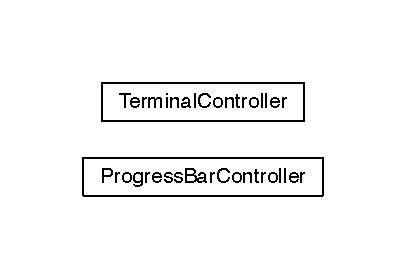
\includegraphics{inheritance-4e77634e702cb303b37f325de087d3f5b165b913.pdf}


\section{Indices and tables}
\label{\detokenize{indices::doc}}\label{\detokenize{indices:indices-and-tables}}\begin{itemize}
\item {} 
\DUrole{xref,std,std-ref}{genindex}

\item {} 
\DUrole{xref,std,std-ref}{modindex}

\item {} 
\DUrole{xref,std,std-ref}{search}

\end{itemize}



\renewcommand{\indexname}{Index}
\printindex
\end{document}